\setchapterpreamble[u]{\margintoc}

\chapter{Complementos}
\section{Complementos de la parte 1}
\subsection{Teorema del punto fijo de Brouwer}
Uno de los resultados clásicos de la topología algebraica es el
\textbf{teorema del punto fijo de Brouwer}, de gran importancia en diversas
áreas de las matemáticas tales como la teoría de juegos. La formulación
estándar del teorema de Brouwer (así como la de otros muchos teoremas de punto
fijo de análisis funcional) es la siguiente:

\begin{theorem}[Teorema del punto fijo de Brouwer]
Sea $D$ una bola cerrada y  $f: D^n \to D^n$ una función continua. Existe un
$p \in D$ tal que $f(p)=p$.
\end{theorem}

\begin{proof}
Supongamos que $f$ no posee puntos fijos:
\[\forall x\in D^n \quad f(x)\neq x \iff \|x-f(x)\| > 0\]
Consideramos entonces la semirrecta
\begin{align*}
r_x=\{\mu u(x)+x: \mu \geq 0\}; && u(x)=\frac{x-f(x)}{\|x-f(x)\|}
\end{align*}
Se define la correspondencia $g\colon D \to \p D$ que asigna a $x$ un
punto $g(x)\in r_x\cap \p D$.

\begin{marginfigure}
\resizebox{\textwidth}{!}{
\begin{tikzpicture}
\draw (0,0) circle (2cm);				

\draw[-to] (.8,.8) -- (-2,-2);
\draw[fill=green] (.8,.8) circle (2pt);
\draw[fill=green] (-.4,-.4) circle (2pt);
\draw[fill=green] (-1.42,-1.42) circle (2pt);

\draw[stealth-stealth] (-3,0) -- (3,0);
\draw[stealth-stealth] (0,-3) -- (0,3);
	
\draw (1.2,.6) node {$f(x)$};
\draw (-.4,-.8) node {$x$};
\draw (-2,-1.42) node {$g(x)$};
\end{tikzpicture}
}
\caption[Aplicación $g$ ilustrada.]{La aplicación $g$ extiende una semirrecta
que pasa por los puntos $x$ y $f(x)$ para tomar el punto de intersección
con la esfera unidad. Dicho punto de intersección es $g(x)$.}
\end{marginfigure}

Queremos ver que $g(x)$ es un singulete. Dados dos puntos $p,q \in r_x$,
existen $\lambda, \mu \geq 0$ tales que
\[p=u_x\mu+x; \quad q=u(x)\lambda+x \implies p-q=u(x)(\mu-\lambda)\]
Tomando normas a ambos lados de la igualdad,
\[\|p-q\|=|\mu-\lambda|\|u(x)\|=|\mu-\lambda|\]
de lo que se deduce que no hay dos puntos diferentes con la misma norma. Por
tanto, $g$ es una aplicación continua.

Observar que, si $x \in \p D$, será el único punto de $r_x$ con norma $1$.
De aquí se sigue que $g$ fija los puntos de $\p D$, por lo que es un retracto
fuerte e induce un epimorfismo
\[g_*\colon H_n(D) \longrightarrow H_n(\p D)\]

Como $D$ es convexo, $H_n(D)$ es un grupo trivial para todo $n > 0$; no
obstante, $\p D$ es homeomorfo a un cierto $S^n$, por lo que $H_n(\p D)$
tiene rango 1. Dado que $g_*$ es sobreyectiva, si llamamos $\alpha$ al
generador de $H_n(\p D)$, existirá un $b \in H_n(\p S)$ tal que $f(b)=\alpha$.

Dado que $b \in H_n(D)=0$, se tiene que $\alpha=f(b)=0$, en contradicción
con el hecho de que $\alpha$ es un generador de un grupo no trivial. Por tanto,
existe un $x \in D$ tal que $f(x)=x$.
\end{proof}

\subsection{Grado de Brouwer}
Sean $n \geq 1$ y $f\colon S^n \to S^n$ una aplicación continua no nula. Dado
un generador $\alpha \in H_n(S^n)$, $f_*(\alpha)=m\alpha$ para algún
$m\neq 0$. Este valor es independiente del $\alpha$ que hemos elegido, dado
que
\[f_*(-\alpha)=m(-\alpha)=-(m\alpha)=-f_*(\alpha)\]
por lo que podemos identificar $m$ con $f$. Este valor se denota como $d(f)$
\footnote{No confundir con la diferencial de una aplicación diferenciable.}
y se denomina \textbf{grado de Brouwer} de $f$.

El grado de Brouwer tiene las siguientes propiedades fundamentales:
\begin{enumerate}
\item Si $f$ es la identidad, $d(f)=1$.
\item Dados $S^n \xrightarrow{f} S^n \xrightarrow{g} S^n$, $d(f\circ g)=
d(f)d(g)$.
\item Si $f$ es constante, $d(f)=0$.
\item Dados $S^n \xrightarrow{f} S^n \xrightarrow{g} S^n$, $f$ es homotópica
a $g$ si y sólo si $d(f)=d(g)$.
\item La aplicación $f$ es una equivalencia de homotopía si y sólo si $d(f)$
es $\pm 1$.
\end{enumerate}

Dada una apliación $f\colon S^n \to S^n$, consideramos la aplicación
$\Sigma f\colon S^{n+1}\to S^{n+1}$ dada por
\[\Sigma f(x,t)=
\begin{cases}
(0,t)				& \text{if $x=0$}\\
(\|x\|f(x/\|x\|),t)	& \text{if $x\neq 0$}
\end{cases}\]
donde $(x,t) \in \mb{R}^{n+1}\times\mb{R}$ verifica que $\|x\|^2+|t|=1$. Esta
aplicación se denomina \textbf{suspensión} de $f$.

\begin{proposition}
Si $f\colon S^n \to S^n$ verifica que $n > 0$, $d(\Sigma f)=d(f)$.
\end{proposition}

Para poder visualizar la suspensión de $f$, consideramos $S^n$ como el ecuador
de $S^{n+1}$. Dado un $t \in [-1,1]$, si $S_t^n$ es el subespacio de $S^{n+1}$
dado por $x_{n+2}=t$, la aplicación
\begin{diag}
\phi_t\colon S^n \arrow[r] & S^n_t\\[-8mm]
			x \arrow[maps to,r] &(\left[1-t\right]x,t)
\end{diag}
es un homeomorfismo y verifica que
\[\Sigma f|_{S^n_t}=\phi_t\circ f\circ \phi_t^{-1}\]

\begin{proposition}
Sean $n > 0$ y $f\colon S^n \to S^n$ la aplicación
\[f(x_1,\dots,x_{n+1})=(-x_1,x_2,\dots,x_{n+1})\]
Entonces, $d(f)=-1$.
\end{proposition}

\begin{proof}
Consideremos el caso $n=1$. Sean $N=(0,1)$, $S=(0,-1)$ y $W=(-1,0)$,
$E=(1,0)$. Entonces, $f$ es Mayer-Vietoris continua bajo el recubrimiento
$U=S^1\backslash \{S\}$, $V=S^1\backslash \{N\}$.

Sea $f_3=f|_{U\cap V}$. El diagrama
\begin{diag}
0 \arrow[r] & H_1(S^1) \arrow{r}{\Delta} \arrow{d}{f_*} & H_0(U\cap V)
	\arrow{d}{f_{3*}}\\
0 \arrow[r] & H_1(S^1) \arrow{r}{\Delta} & H_0(U\cap V)
\end{diag}
tiene filas exactas, y el rectángulo es conmutativo. Un generador $\alpha$ de
$H_1(S^1)$ se puede representar como un ciclo en la forma $c+d$, donde
$\p c=x-y=-\p d$, en cuyo caso $\Delta(\alpha)=x-y$. Ahora bien,
\[(\Delta\circ f_*)(\alpha)=(f_{3*}\circ \Delta)(x)=f_{3*}(x-y)=y-x=
-\Delta(\alpha)=\Delta(-\alpha)\]
Dado que $\Delta$ es un monomorfismo, $d(f)=-1$.

Asumamos ahora que $d(f)=-1$ para $n-1 \geq 1$. Consideramos $S^{n-1}$ como el
subespacio de $S^n$ dado por la ecuación $x_{n+1}=0$, de forma que $S^{n-1}$ es
el ecuador de $S^n$. Tomamos $U=S^n\backslash \{N\}$ y $V=S^n\backslash \{S\}$,
siendo $N=(0,\dots,0,1)$ y $S=(0,\dots,0,-1)$. Con esta notación, la inclusión
\[i\colon S^{n-1}\hookrightarrow U\cap V\]
es una equivalencia de homotopía.

Dado que $n > 1$, el homomorfismo de conexión $\Delta$ es un homomorfismo. Por
tanto, tenemos el doble diagrama conmutativo
\begin{diag}
H_n(S^n) \arrow{r}{\Delta} \arrow{d}{f_*} & H_{n-1}(U\cap V)
	\arrow{d}{f_{3*}} & H_{n-1}(S^{n-1}) \arrow[swap]{l}{i_*} \arrow{d}{f_*}\\
H_n(S^n) \arrow{r}{\Delta} & H_{n-1}(U\cap V) & H_{n-1}(S^{n-1})
	\arrow[swap]{l}{i_*}
\end{diag}
donde las filas describen isomorfismos. Si llamamos $\alpha$ al generador de
$H_n(S^n)$,
\begin{align*}
f_*(\alpha)&=(\Delta^{-1}\circ f_{3*}\circ \Delta)(\alpha)
=(\Delta^{-1}\circ i_*\circ f_{3*}\circ i_*^{-1}\circ \Delta)(\alpha)=\\
&=-(\Delta^{-1}\circ i_*\circ i_*^{-1}\circ \Delta)(\alpha)=-\alpha
\end{align*}
\end{proof}

Como consecuencia de este resultado, si $f$ cambia el signo de $1 \leq j\leq
n$ componentes, $d(f)=(-1)^j$. En particular, la aplicación antipodal
$A(x)=-x$ tiene grado de Brouwer $(-1)^n$.

\begin{proposition}\labprop{Antipodal}
Si $f,g\colon S^n \to S^n$ son aplicaciones con $f(x)\neq g(x)$ para todo $x$,
$g$ es homotópica a $A\circ f$.
\end{proposition}

\begin{proof}
Dado que $f(x)\neq g(x)$, el segmento
\[L=\{tA[f(x)]+(1-t)g(x)\colon t \in [0,1]\}\]
no contiene al punto $0$. Por tanto, la homotopía $F\colon S^n\times I \to
S^n$ dada por
\[F(x,t)=\frac{tA[f(x)]+(1-t)g(x)}{\|tA[f(x)]+(1-t)g(x)\|}\]
está bien definida.
\end{proof}

\begin{marginfigure}
\resizebox{\textwidth}{!}{
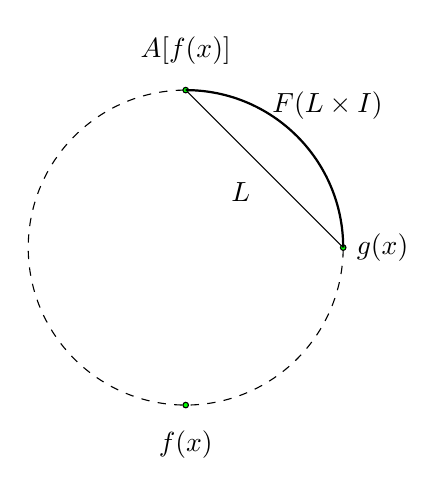
\begin{tikzpicture}
	\draw (2,0) -- (0,2);
	\draw[dashed] (0,0) circle (2cm);
	\draw (0.7,0.7) node {$L$};
	
	\draw[fill=green] (2,0) circle (1pt);
	\draw (2.5,0) node {$g(x)$};

	\draw[fill=green] (0,2) circle (1pt);
	\draw (0,2.5) node {$A[f(x)]$};

	\draw[fill=green] (0,-2) circle (1pt);
	\draw (0,-2.5) node {$f(x)$};
	
	\draw[thick] (2,0) arc (0:90:2cm);
	\draw (1.8,1.8) node {$F(L\times I)$};

\end{tikzpicture}
}

\caption{Representación gráfica de la \refprop{Antipodal}.}
\end{marginfigure}

Consideremos una $f\colon S^{2n} \to S^{2n}$ continua. Si $f(x)\neq x$ para
todo $x$, $f$ es homotópica a $A=A\circ \id_{S^{2n}}$ y
\[d(f)=d(A)=(-1)^{2n+1}\]
Si suponemos que $f(x)\neq -x$ para todo $x$, $f$ es homotópica a
$\id_{S^{2n}}=A\circ A$ y
\[d(f)=d(\id)=1\]
Dado que $d(f)$ es único, debe pasar que $f(x)=x$ ó $f(x)=-x$ para algún
$x \in S^{2n}$.

\begin{corollary}[Teorema de la bola peluda]
Dada $f\colon S^{2n} \to S^{2n}$ continua, $f(x)$ no puede ser ortogonal a $x$
para todo $x$. Por tanto, todo campo vectorial sobre $S^{2n}$ es nulo.
\end{corollary}

\section{Complementos de la parte 2}
